\documentclass[UTF8, onecolumn, a4paper]{article}
\usepackage{ctex}
\usepackage{appendix}
\usepackage{geometry}
\usepackage{amsmath, amsthm}
\usepackage{multirow, multicol}
\usepackage{subfigure}
\usepackage{float}
\usepackage{graphicx}
\usepackage{lettrine}
\usepackage{authblk}
\usepackage{xcolor, fontspec}%用于设置颜色
\usepackage[ruled,vlined]{algorithm2e}
\usepackage{listings}%用于显示代码
\usepackage{amssymb}
\geometry{left=3.0cm,right=3.0cm,top=2.0cm,bottom=2.0cm}

\title{\textbf{《图论与代数结构》部分习题解析}}%———总标题
\author{刘泓尊\quad 2018011446\quad 计84
	\\ \texttt{liu-hz18@mails.tsinghua.edu.cn}}
\affil{Department of Computer Science and Technology, Tsinghua University}

\begin{document}
\maketitle 
\lstset{%代码块全局设置
	backgroundcolor=\color{red!3!green!3!blue!3},%代码块背景色为浅灰色
	rulesepcolor= \color{gray}, %代码块边框颜色
	breaklines=true,  %代码过长则换行
	numbers=left, %行号在左侧显示
	numberstyle= \small,%行号字体
	%keywordstyle= \color{red},%关键字颜色
	commentstyle=\color{gray}, %注释颜色
	frame=shadowbox,%用方框框住代码块
	xleftmargin=1em,
	xrightmargin=0em,
	tabsize=5,
	%rulesepcolor=\color{red!20!green!20!blue!20},  %阴影颜色
	keywordstyle={\color{blue!90!}\fontspec{Consolas Bold}},   %关键字颜色
	commentstyle={\color{blue!70!black}\fontspec{Consolas Italic}},   %注释颜色
	stringstyle=\color{orange!100!black}, %字符串颜色
	numberstyle=\color{purple}, %行号颜色
	%basicstyle=\ttfamily, %代码风格
	basicstyle=\fontspec{Consolas},
	showstringspaces=false,          % underline spaces within strings only  
	showtabs=false,
	captionpos=t, %文件标题位置
	flexiblecolumns
}

\begin{description}
\section*{Chapter 1}
\item[1.] 
\begin{proof}
以工厂为节点,工厂之间有联系则建边,构成无向图。\\
a.假设每座工厂都只与其他3座工厂有联系,则总度数为
$$\underset{v\in V(G)}{\sum}d(v) = 9 \times 3 = 27$$
由性质1.1.1,图的度数和应为偶数,矛盾!\\
故,不可能每座工厂都只与其他三座工厂有业务联系。\\
b.假设只有4座工厂与偶数个工厂有业务联系,剩余5个工厂与奇数个工厂有联系,则总度数为
$$\underset{v\in V(G)}{\sum}d(v) = 4 \times 2i + 5 \times(2j+1) = 2(4i+5j)+1$$
上式为奇数,同样与性质1.1.1矛盾!\\
故,不可能只有4座工厂与偶数个工厂有联系.
\end{proof}
\item[2.] 
\begin{proof}
	假设$G$中存在至少1个孤立节点,则至多有$n-1$个非孤立节点。由于$G$为简单图,不存在重边和自环,所以每个非孤立节点最多与$n-2$个非孤立节点相连,总边数
	$$m = \frac{1}{2}\underset{v\in V(G)}{\sum}d(v) \leq \frac{1}{2}\underset{v\in V(G)}{\sum}(n-2) \leq \frac{1}{2}(n-1)(n-2)$$
	与题设条件$$m > \frac{1}{2}(n-1)(n-2)$$矛盾!\\
	故,$G$中不存在非孤立节点。
\end{proof}
\item[3.]
\begin{proof}
根据定义,有向完全图满足条件
$$d^+(v_i)+d^-(v_i) = n-1,\quad v_i\in V(G)$$
故
\begin{equation}
\begin{aligned}
left - right &=
\underset{v_i\in V(G)}{\sum}\left((d^+(v_i))^2 - (d^-(v_i))^2\right)\\ &= 
\underset{v_i\in V(G)}{\sum}\left((d^+(v_i))^2 - (n-1-d^+(v_i))^2\right)\\
&=\underset{v_i\in V(G)}{\sum}\left(2(n-1)d^+(v_i) - (n-1)^2\right)\\
&=2(n-1)\underset{v_i\in V(G)}{\sum}d^+(v_i) - n(n-1)^2\\
&=2(n-1)\frac{n(n-1)}{2} - n(n-1)^2\\
&=0
\end{aligned}
\end{equation}
即
$$\underset{v_i\in V(G)}{\sum}(d^+(v_i))^2 = \underset{v_i\in V(G)}{\sum}(d^-(v_i))^2$$
\end{proof}

\item[4.]
设$8L,5L,3L$的容器对应节点$(a,b,c)$,其中$a,b,c$分别依次对应三种容器。\\
搜索思路:\\
对状态进行转移与搜索(dfs),当某一容器m非空且存在另一容器n不满时,就可以将水从m倒入n中,使得m空或者n满,以此作为一次状态转移;\\
对各状态进行DFS之后可以得到如下图所示的解。解的路径就是操作的具体过程。\\
\begin{figure}[h]
	\centering
	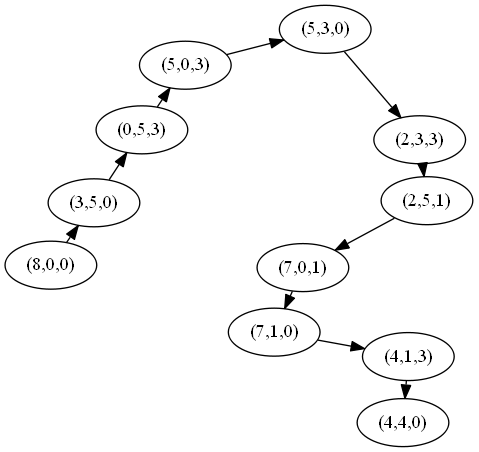
\includegraphics[width=0.70\textwidth]{demo.png}
\end{figure}
$\bullet$附录(Appendix)给出了具体实现代码。

\item[7.]
同构。构造映射$f:G_a\rightarrow G_b$如下:
\begin{center}
	\begin{tabular}{ccccccc}
	\hline
		$v$ & $v_1$ & $v_2$ & $v_3$ &  $v_4$ & $v_5$ & $v_6$\\
	\hline
		$f(v)$&b & a& c & e & d & f  \\
	\hline
	\end{tabular}
\end{center}
\item[8.]\quad\\
邻接矩阵:
\begin{center}
$\begin{pmatrix}
	0 & 1 & 0 & 1 & 0 & 0\\
	0 & 0 & 0 & 0 & 1 & 0\\
	1 & 0 & 0 & 1 & 0 & 0\\
	0 & 0 & 0 & 0 & 0 & 0\\
	0 & 0 & 1 & 0 & 0 & 0\\
	1 & 0 & 1 & 1 & 0 & 0
\end{pmatrix}$
\end{center}
设边的顺序为$e_1 = (v_1, v_2), e_2 = (v_1, v_4), e_3 = (v_3, v_1), e_4 = (v_2, v_5), e_5 = (v_6, v_3), e_6 = (v_6, v_4), e_7 = (v_5, v_3), e_8 = (v_3, v_4), e_9 = (v_6, v_1)$\\
关联矩阵:
\begin{center}
$\begin{pmatrix}
1 & 1 & -1 & 0 & 0 & 0 & 0 & 0 & -1\\
-1 & 0 & 0 & 1 & 0 & 0 & 0 & 0 & 0\\
0 & 0 & 1 & 0 & -1 & 0 & -1 & 1 & 0 \\
0 & -1 & 0 & 0 & 0 & -1 & 0 & -1 & 0 \\
0 & 0 & 0 & -1 & 0 & 0 & 1 & 0 & 0\\
0 & 0 & 0 & 0 & 1 & 1 & 0 & 0 & 1
\end{pmatrix}$
\end{center}
边列表:
$$A = (1, 1, 3, 2, 6, 6, 5, 3, 6)$$
$$B = (2, 4, 1, 5, 3, 4, 3, 4 ,1)$$
正向表:
$$A = (1, 3, 4, 6, 6, 7, 10)$$
$$B = (2, 4, 5, 1, 4, 3, 3, 4 ,1)$$

\section*{Chapter 2}
\item[Thinking.]
完全二分图$K_{m, n}$何时为欧拉图?\\
由于无向连通图$G$存在欧拉回路(是欧拉图)的充要条件是$G$中每个节点的度均为偶数。\\
而完全二分图两子集$X, Y$中,$X$中节点度为$|Y|$,$Y$中节点度为$|X|$,故充要条件为:
\begin{center}
	$m, n$均为偶数
\end{center}

\item[2.]
\begin{proof}
假设$G$和$\overline{G}$均不是连通图\\
设$G$存在连通支$G_1, G_2$,在$G$中任取节点$v_1, v_2$:\\
$\bullet$若存在边$(v_1, v_2)$,则在$G_2$中取点$v_3$,$v_3$与$v_1,v_2$均不连通,由补图的定义,$\overline{G}$中$v_3$与$v_1, v_2$连通,则$\overline{G}$中$v_1$与$v_2$通过$v_3$连通。\\
$\bullet$若不存在边$(v_1, v_2)$,则由补图的定义,$\overline{G}$中$v_1$与$v_2$通过$v_3$连通.\\
由$v_1, v_2$的任意性知,$\overline{G}$连通。与假设矛盾!\\
故$G$和$\overline{G}$至少有一个是连通图。
\end{proof}

\item[3.]
\begin{proof}
图$G$有两条最长道路$L_1, L_2$,其长度均为$l$,假设两条道路不相交,即两者没有公共顶点\\
由于$G$为连通图,$L_1,L_2$中分别存在点$v_1, v_2$使得存在$v_1\rightarrow v_2$的道路,设该道路为$L$.\\
$v_1$分$L_1$为两部分,一部分$L_{1a}$长度$\geq l/2$;同理,$v_2$分$L_2$为两部分,一部分$L_{2a}$长度$\geq l/2$,则取道路$L_{1a} \cup L_{2a} \cup L$,该道路长度$\geq l/2+l/2+1 = l+1$,与$L_1, L_2$是最长道路的假设矛盾!\\
故若连通图最长道路不唯一,它们必定相交。
\end{proof}

\item[4.]
\begin{proof}
对顶点数n作归纳。\\
\textbf{a.}$n = 4$时,$m\geq5$。\\
若$G$中存在度为0或1的节点,则剩余3个节点的子图的度$\sum deg \geq4$,与简单图的边数矛盾。故$G$中节点$deg\geq2$.则$G$中回路只有两种形式:
\begin{center}
	\quad1.三角形回路\quad2.四边形回路
\end{center}
$\bullet$若为三角形回路,则$G$中剩下的一个顶点至少与此三角形有2条边,这两条边与原三角形两边构成四边形回路,三角形剩下的一条边就是弦$(Chord)$.\\
\qquad$\bullet$若为正方形回路,则至少还有一条边,该边就是弦。\\
\textbf{b.}假设对节点数$n-1$的图成立.\\
\textbf{c.}对于节点数为$n$的图:\\
\qquad$\bullet$若$G$中存在度为1的节点$v$,则将该节点及其所连边去除后,由归纳假设知命题成立.\\
\qquad$\bullet$若$G$中存在度为2的节点$v$,设该节点所连点为$v_s, v_t$,则去除$v$及其所连边,并将$v_s, v_t$合并为一个节点,该图即为$n-1$的图$G'$,由归纳假设知$G'$存在带弦回路,还原为$G$后仍然是带弦回路。\\
\quad$\bullet$否则,$G$中所有节点$deg\geq 3$,由例$2.1.3$结论可知,$G$中必含带弦回路。
\end{proof}

\item[6.]
\begin{proof}[解]
将图中房间设为顶点,同时增设外部节点$Out$,两节点之间边代表有门;构造新图$G$如下.\\
问题转化为$G$中是否存在欧拉道路,由于$G$中存在度为奇的两个点$v_3,v_5$,由推论2.3.1得$G$中存在欧拉道路,所以存在一条路经过每个门一次。
\begin{figure}[h]
	\centering
	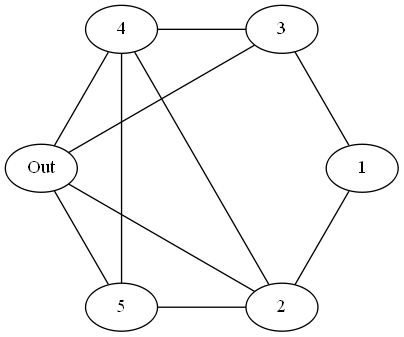
\includegraphics[width=0.35\textwidth]{demo2.png}
\end{figure}
\end{proof}

\item[8.]
\begin{proof}
假设$G$不存在$H$回路,则由推论2.4.1,存在节点$v_i, v_j$使得$d(v_i) + d(v_j) < n$.\\
考虑图$G' = G - {v_i, v_j}$,即图$G$删去节点$v_i, v_j$及其所连边的情况.\\
一方面,$$m_{G'} = m - (d(v_i) + d(v_j)) > m - n \geq \frac{1}{2}(n-1)(n-2) + 2 - n = \frac{1}{2}(n-2)(n-3)$$
另一方面,
$$m_{G'} < m_{K_{n-2}} = \frac{1}{2}(n-2)(n-3)$$
上述两式矛盾,所以$G$中存在$H$回路。
\end{proof}

\item[12.]
\begin{proof}
不能.\\
将正方体的27个节点建模为二分图(或2-染色),具体做法为:\\8个顶点和6个面的中心点归为点集$X$,12条棱中点和体中心点归为点集$Y$,那么相邻节点之间必为一个$X$,一个$Y$。\\
而一个角的顶点为$X$,中心为$Y$,根据二分图的性质,从点集$X$走到点集$Y$中所经过路径长度必然为奇数;而遍历27个顶点仅一次只需要26步,是偶数,矛盾!\\
所以不能实现.
\end{proof}

\item[14.]
\begin{proof}[解]
将4个坐标点连同原点建图,以坐标为节点,坐标之间的曼哈顿距离为边权,构建完全图$K_5$,如下图所示\\
\begin{figure}[h]
	\centering
	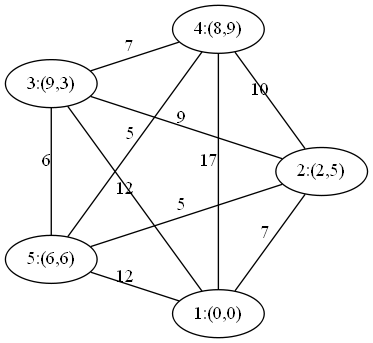
\includegraphics[width=0.4\textwidth]{demo3.png}
\end{figure}
问题转化为求下图的最短哈密顿回路,即TSP,采用分支与界法可以求得问题的解。\\
1.将边权递增排序,初始界$d_0\leftarrow\infty$\\
\begin{center}
	\begin{tabular}{ccccccccccc}
		\hline
		$e_{ij}$ & $a_{25}$ & $a_{45}$ & $a_{35}$ &  $a_{12}$ & $a_{34}$ & $a_{23}$ & $a_{24}$ & $a_{13}$ & $a_{15}$ & $a_{14}$ \\
		\hline
		$w_{ij}$& 5 & 5 & 6 & 7 & 7 & 9 & 10 & 12 & 12 & 17\\
		\hline
	\end{tabular}
\end{center}
2. 边权序列 中依次选边进行$dfs$,直到选择$n$条边,判断是否构成$H$回路.
\\求解过程如下:\\
$\bullet$\quad$d(S_1) = d(a_{25}, a_{45}, a_{35}, a_{12}, a_{34}),$ it's not a $Hamiltonian\quad Circle$. if $a_{34}$ is replaced by $a_{23}, a_{24}, a_{13}, a_{15}, a_{14}$, it's still not a $Hamiltonian\quad Circle$. Likely, if $a_{12}$ is replaced by $a_{34} ,a_{23}, a_{24}, a_{13}, a_{15}$, it's still not a $Hamiltonian\quad Circle$.\\
$\bullet$\quad$ d(S_2) = d(a_{25}, a_{45}, a_{12}, a_{34}, a_{23})$, it's not a $Hamiltonian\quad Circle$. Until\\ $d(S_3) = d(a_{25}, a_{45}, a_{12}, a_{34}, a_{13}) = 36$ , it's a $Hamiltonian\quad Circle$, $d_0\leftarrow36$.\\
$\bullet$\quad$d(S_4) = d(a_{25}, a_{45}, a_{34}, ..., ...)$ are all not a  $Hamiltonian\quad Circle$.\\
$\bullet$\quad$d(S_5) = d(a_{25}, a_{35}, a_{12}, a_{34}, a_{14}) = 42$, it's a $Hamiltonian\quad Circle$.\\
类似的,继续进行下去得到的解会比36大,所以TSP问题的解是$$d(S_3) = d(a_{25}, a_{45}, a_{12}, a_{34}, a_{13}) = 36$$即行进路线为:
$$(0, 0)\rightarrow(2, 5)\rightarrow(6, 6)\rightarrow(8 ,9)\rightarrow(9, 3)\rightarrow(0,0)$$
最短路径长36.
\end{proof}
\item[15.]
\begin{proof}[解]
可以将5年的6个时间点看做节点,节点之间的有向边代表1台设备从一年用到另一年的总花费,形成$DAG$,最小花费即为该图从起点到终点的最短路径,使用最短路算法可以解决这个问题。1台设备累计花费为费用数组的前缀和,即$(1, 3, 6, 11, 17)$,建图如下:
\begin{figure}[h]
	\centering
	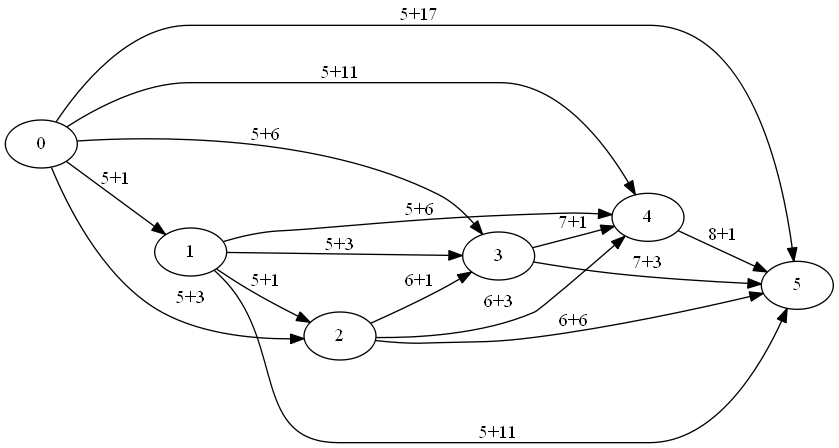
\includegraphics[width=0.9\textwidth]{demo4.png}
\end{figure}
\\对上图使用最短路算法,得到的最短路如下:
\begin{figure}[h]
	\centering
	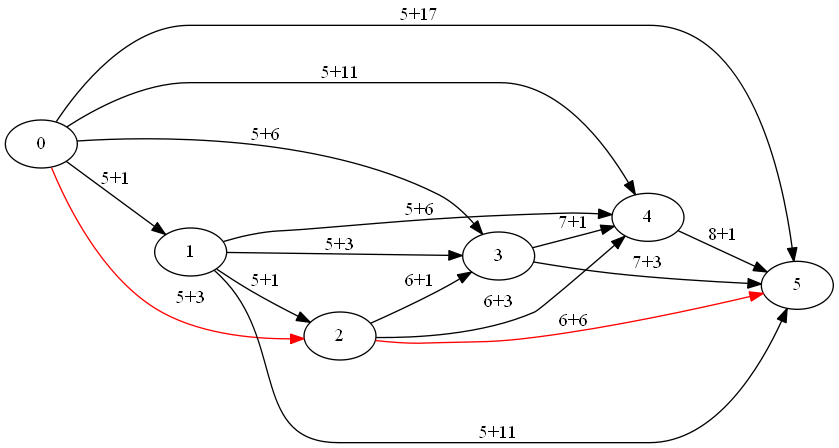
\includegraphics[width=0.9\textwidth]{demo5.png}
\end{figure}
\\所以最少开支的方案为:\\
第1年购买1台设备使用2年(花费5+1+2 = 8),第3年购买1台设备使用3年(花费6+1+2+3 = 12)。总开支20。
\end{proof}

\item[16.]
\begin{proof}[解]
采用$Edmonds$最小权匹配求解中国邮路。
\begin{figure}[h]
	\centering
	\subfigure{
		\begin{minipage}[t]{0.3\linewidth}
			\centering
			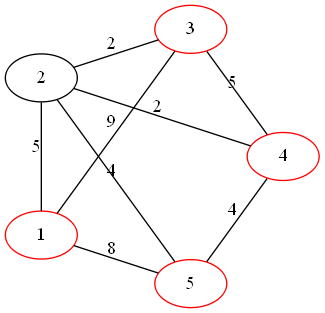
\includegraphics[width=\textwidth]{demo7.png}
			\caption{deg为奇}
		\end{minipage}
	}
	\subfigure{
		\begin{minipage}[t]{0.3\linewidth}
			\centering
			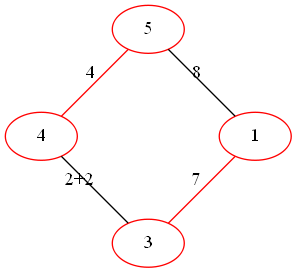
\includegraphics[width=\textwidth]{demo9.png}
			\caption{最小权匹配}
		\end{minipage}
	}
	\subfigure{
		\begin{minipage}[t]{0.3\linewidth}
			\centering
			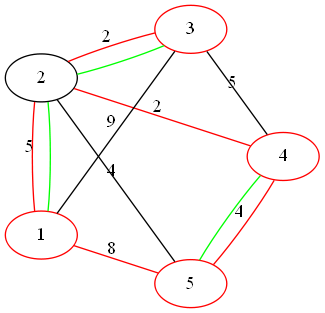
\includegraphics[width=\textwidth]{demo8.png}
			\caption{中国邮路}
		\end{minipage}
	}
\end{figure}
\\1.找到图中度为奇的节点(图中红色节点)。\\
2.对图中红色节点寻找在原图中的最短路,进行最小权匹配(图中红色边为选中的边)。\\
3.将最小权匹配中选择的边设置为重边(图中绿色边),得到欧拉图$G'$.\\
4.\quad$G'$的一条欧拉回路就是解。\\
\textbf{Conclusion}:中国邮路长度为$d = 50$,重复走的边为$1-2,2-3,4-5$.
\end{proof}

\item[17.]
\begin{proof}[解]
工序的PT图如下图所示:
\begin{figure}[h]
	\centering
	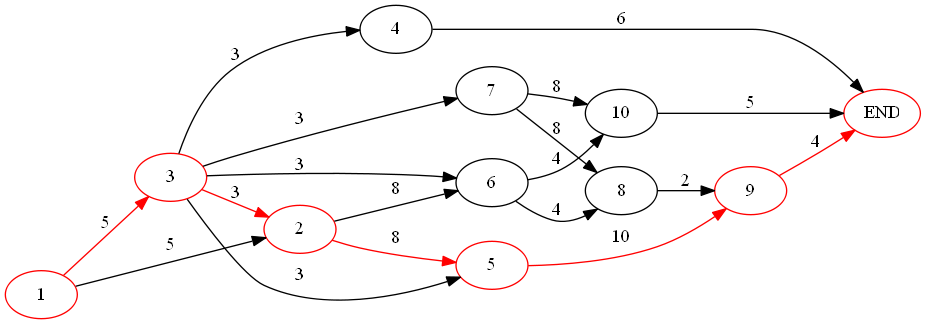
\includegraphics[width=0.9\textwidth]{demo6.png}
\end{figure}
\\对上图使用拓扑排序算法,得到工序的拓扑序为:
\begin{center}
	\begin{tabular}{cccccccccccc}
		\hline
		TopoRank &1 & 2 & 3 & 4 & 5 & 6 & 7 & 8 & 9 & 10 & 11\\
		\hline
		Vertex&1& 3& 7& 4 & 2 & 6 &10 &8&5&9& $END$ \\
		\hline
	\end{tabular}
\end{center}
关键路径如上图红色路径所示。\\得到工序3,5,10的最早启动时间为$$\pi(3) = 5, \pi(5) = 16, \pi(10) = 20$$
最晚启动时间为$$\tau(3) = 5, \tau(5) = 16, \tau(10) = 25$$
允许延误时间为$$t_3 = 0, t_5 =0,t_{10}=5$$
\end{proof}

\item[Thinking.]
$\frac{1}{4}$国际象棋棋盘跳马问题?
\begin{proof}
原问题可转化为求解下图的哈密顿回路问题:
\begin{figure}[h]
	\centering
	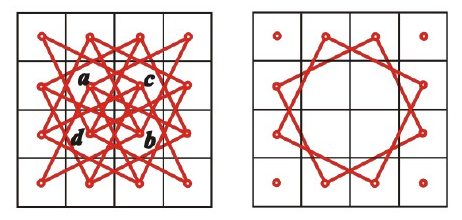
\includegraphics[width=0.6\textwidth]{demo10.png}
\end{figure}
\\如图,删去$S=\{a,b,c,d\}$四个点,得到$G-S$.因为$$p(G-S) = 6 > |S| = 4$$故该图不存在哈密顿回路,所以跳马问题无解。
\end{proof}

\section*{Chapter 3}
\item[1.]
\begin{proof}[解]
设树有$n_1$个度为1的节点,总节点数为$n$,$k\geq3$时,由树的性质:
$$n_1 + 2n_2 + 3n_3 + \cdots + kn_k = 2(n-1)$$
$$n_1+n_2+n_3+\cdots+n_k = n$$
联立以上两式,解得:
$$n_1 = 2 + n_3 + \cdots (k-2)n_k = 2 + \sum_{i=3}^{k}(i-2)n_i,\quad k \geq 3$$
$k=2$时,该树只有1个树根和2个孩子,度为1的节点有$2$个。综上,度为1的节点数:
\begin{equation}
n_1=
\begin{cases}
2&k = 2\\
2 + \sum_{i=3}^{k}(i-2)n_i&k\geq3
\end{cases}
\end{equation}
\end{proof}

\item[4.]
\begin{proof}[解]
\textbf{a.}原图的$Laplacian$矩阵为:
\begin{center}
	$L(G) = \begin{pmatrix}
	3 & -1 & 0 & -1 & -1\\
	-1 & 4 & -1 & 0 & -2\\
	0 & -1 & 4 & -2 & -1 \\
	-1 & 0 & -2 & 4 & -1 \\
	-1 & -2 & -1 & -1 & 5
	\end{pmatrix}$
\end{center}
树的数目为:
$$det(L') = det\left(
\begin{array}{cccc}
3 & -1 & 0 & -1\\
-1 & 4 & -1 & 0\\
0 & -1 & 4 & -2 \\
-1 & 0 & -2 & 4 \\
\end{array}
\right) = 101$$

\textbf{b.}$G/\{v_1,v_5\}$(缩点)的$Laplacian$矩阵:
\begin{center}
	$L(G/\{v_1,v_5\})=\begin{pmatrix}
	6 & -3 & -1 & -2\\
	-3 & 4 & -1 & 0\\
	-1 & -1 & 4 & -2 \\
	-2 & 0 & -2 & 4 
	\end{pmatrix}$
\end{center}
必含$(v_1, v_5)$的树的数目:
$$det(L') = det\left(
\begin{array}{ccc}
6 & -3 & -1\\
-3 & 4 & -1\\
-1 & -1 & 4
\end{array}
\right) =44 $$
\textbf{c.} 
$G-(v_1,v_5)$(删边)的$Laplacian$矩阵:
\begin{center}
	$L(G-(v_1,v_5))=\begin{pmatrix}
	3 & -1 & 0 & -1 & -1\\
	-1 & 4 & -1 & 0 & -2\\
	0 & -1 & 4 & -2 & -1 \\
	-1 & 0 & -2 & 3 & 0 \\
	-1 & -2 & -1 & 0 & 4
	\end{pmatrix}$
\end{center}
不含$(v_4, v_5)$的树的数目:
$$det(L') = det\left(
\begin{array}{cccc}
3 & -1 & 0 & -1\\
-1 & 4 & -1 & 0\\
0 & -1 & 4 & -2 \\
-1 & 0 & -2 & 3
\end{array}
\right) =  60$$
\end{proof}

\item[5.]
\begin{proof}[解]
\textbf{a.}原图的$Laplacian$矩阵为:
\begin{center}
	$L(G) = \begin{pmatrix}
	0 & -1 & 0 & -1 & -1\\
	0 & 2 & -1 & 0 & -1\\
	0 & 0 & 3 & -1 & 0 \\
	0 & 0 & -1 & 3 & 0 \\
	0 & -1 & -1 & -1 & 2
	\end{pmatrix}$
\end{center}
以$v_1$为根的根树的数目为:
$$det(L') = det\left(
\begin{array}{cccc}
 2 & -1 & 0 & -1\\
 0 & 3 & -1 & 0 \\
 0 & -1 & 3 & 0 \\
 -1 & -1 & -1 & 2
\end{array}
\right) = 24$$

\textbf{b.}$G-(v_1,v_5)$(删边)的$Laplacian$矩阵:
\begin{center}
	$L(G-(v_1,v_5))=
	\begin{pmatrix}
	0 & -1 & 0 & -1 & 0\\
	0 & 2 & -1 & 0 & -1\\
	0 & 0 & 3 & -1 & 0 \\
	0 & 0 & -1 & 3 & 0 \\
	0 & -1 & -1 & -1 & 1 
	\end{pmatrix}$
\end{center}
以$v_1$为根,不含$(v_1, v_5)$的根树的数目:
$$det(L') = det\left(
\begin{array}{cccc}
 2 & -1 & 0 & -1\\
 0 & 3 & -1 & 0 \\
 0 & -1 & 3 & 0 \\
 -1 & -1 & -1 & 1 
\end{array}
\right) = 8 $$
\textbf{c.} 
$G-(v_2,v_3)$(删边)的$Laplacian$矩阵:
\begin{center}
	$L(G-(v_2,v_3))=\begin{pmatrix}
	0 & -1 & 0 & -1 & -1\\
	0 & 2 & 0 & 0 & -1\\
	0 & 0 & 2 & -1 & 0 \\
	0 & 0 & -1 & 3 & 0 \\
	0 & -1 & -1 & -1 & 2
	\end{pmatrix}$
\end{center}
不含$(v_2, v_3)$的树的数目:
$$det(L') = det\left(
\begin{array}{cccc}
2 & 0 & 0 & -1\\
0 & 2 & -1 & 0 \\
0 & -1 & 3 & 0 \\
-1 & -1 & -1 & 2
\end{array}
\right) =  15$$
必含$(v_2, v_3)$的,以$v_1$为根的根树的数目$$24 - 15 = 9$$
\end{proof}

\item[8.]
\begin{proof}
完全二分图$K_{m,n}$的$Laplacian$矩阵:
\begin{center}
	$L(G) = \begin{pmatrix}
	nI_m & -B\\
	-B^T & mI_n
	\end{pmatrix}$
\end{center}
其中$B$为$(m\times n)$的全1矩阵。\\
树的数目为:
\begin{equation}
\begin{aligned}
det(L_{m+n,m+n}) &= det\left(nI_m\right)\cdot det\left(mI_n - B^T\frac{1}{n}I_{n-1}B\right) \\&= n^m\cdot det
\begin{pmatrix}
m - \frac{m}{n} & -\frac{m}{n} & \cdots & -\frac{m}{n} \\
-\frac{m}{n} & m - \frac{m}{n} & \cdots & -\frac{m}{n}\\
\vdots & \vdots & \ddots & \vdots \\
-\frac{m}{n}& -\frac{m}{n} & \cdots& m - \frac{m}{n}
\end{pmatrix} \\&= n^m\cdot \frac{m^{n-1}}{n} \\&= n^{m-1}m^{n-1}
\end{aligned}
\end{equation}
\end{proof}

\item[10.]
\begin{proof}[解]
\textbf{1.}
$$B = (B_{11}, B_{12}) = 
\left(\begin{array}{c|c}
\begin{matrix}
-1& 1 &0 &0 \\
1& 0& 1& 0\\
0 &-1& 0& 0 \\
0 &0 &0 &-1
\end{matrix}&
\begin{matrix}
0 &0 &1 &0\\
0& 1& 0& 0\\
-1& 0 &0 &-1\\
1 &-1& 0 &0
\end{matrix}
\end{array}
\right)
$$
$$B_{12}^{-1} = 
\begin{pmatrix}
0& 1 &0 &1 \\
0 &1 &0 &0 \\
1& 0& 0& 0 \\
0& -1& -1& -1
\end{pmatrix}
$$
以$\{e_3,e_4,e_6,e_7\}$为树边的基本回路矩阵:
$$
C_f = (I, -B_{11}^TB_{12}^{-T}) = 
\begin{pmatrix}
1& 0 &0 &0 &-1& -1 &1 &1\\
0 &1 &0 &0 &0 &0 &-1& -1\\
0& 0& 1& 0 &-1& -1& 0& 1\\
0& 0& 0& 1& 1& 0& 0& -1
\end{pmatrix}
$$

\textbf{2.}
$$B = (B_{11}, B_{12}) = 
\left(\begin{array}{c|c}
\begin{matrix}
-1& 0 &0 &0 \\
1& 0& 1& 0\\
0 &-1& 0& -1 \\
0 &1 &-1 &0
\end{matrix}&
\begin{matrix}
1 &0 &1 &0\\
0& 1& 0& 0\\
-1& 0 &0 &0\\
0 &0& 0 &-1
\end{matrix}
\end{array}
\right)$$

$$B_{12}^{-1} = 
\begin{pmatrix}
	0& 0 &-1 &0 \\
	0 &1 &0 &0 \\
	1& 0& 1& 0 \\
	0& 0& 0& -1
\end{pmatrix}$$

以$\{e_2,e_5,e_6,e_8\}$基本割集矩阵:
$$S_f = (B_{12}^{-1}B_{11}, I) = 
	\begin{pmatrix}
	0& 1 &0 &1 &1& 0 &0 &0\\
	1 &0 &1 &0 &0 &1 &0& 0\\
	-1& -1& 0& -1 &0& 0& 1& 0\\
	0& -1& 1& 0& 0& 0& 0& 1
	\end{pmatrix}
$$
\end{proof}

\item[14.]
\begin{proof}[解]
state act as a seat的字频统计:
\begin{center}
	\begin{tabular}{ccccccc}
		\hline
		char &c & e & s & t & ' ' & a\\
		\hline
		count&1& 2& 3& 4 & 4 & 5\\
		\hline
	\end{tabular}
\end{center}
$Huffman$树的构造及对应字符的编码如下:
\begin{figure}[h]
	\centering
	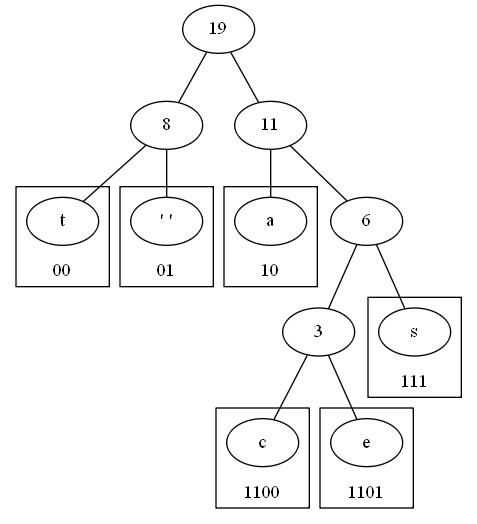
\includegraphics[width=0.5\textwidth]{demo11.png}
\end{figure}
\\二进制编码:
\begin{center}
	\begin{tabular}{ccccccc}
		\hline
		char &c & e & s & t & ' ' & a\\
		\hline
		code&1100& 1101& 111& 00 & 01 & 10\\
		\hline
	\end{tabular}
\end{center}
得到源字符串的$Huffman$编码为:
$$11100100011010110110000011011101100111111011000$$
编码长度$codelen=47$.
\end{proof}

\item[16.]
\begin{proof}[解]
对原图使用$Kruskal$算法,得到的最短树如下:(树边用红色标识)	
\begin{figure}[h]
	\centering
	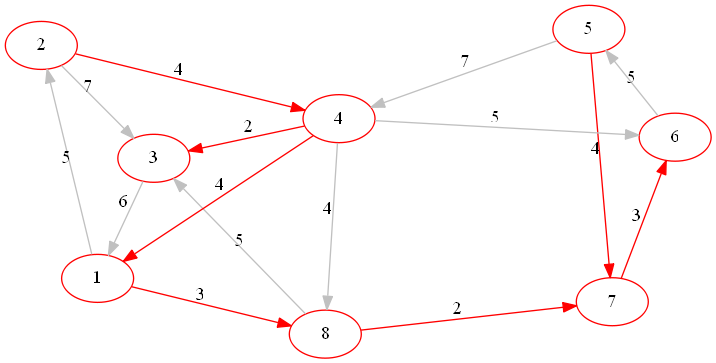
\includegraphics[width=0.8\textwidth]{demo12.png}
\end{figure}	
\\最短树树边为$(v_1,v_8),(v_2,v_4),(v_4,v_1),(v_4,v_3),(v_5,v_7),(v_7,v_6),(v_8,v_7)$,总权$22$.
\end{proof}

\section*{Chapter 4}

\item[3.]
\begin{proof}
假设$G$和$\overline{G}$均为平面图,则
$$|E(G)| \leq 3n-6$$
$$|E(\overline{G})| \leq 3n-6 $$
故$$|E(G)| + |E(\overline{G})| = |E(K_n)| = \frac{n(n-1)}{2}\leq6n-12$$
解得$$3\leq n\leq 10$$
与$n > 10$矛盾!\\所以节点数大于10的简单图中,$G$和$\overline{G}$至少有一个是非平面图。
\end{proof}

\item[7.]
\begin{proof}
假设存在这样的平面图$G$满足题设性质。\\
由于$G$为平面图,则其存在唯一的对偶图$G^*$。根据题设,$G^*$有5个节点,两两节点之间至少有一个边,即$G^*$存在$K_5$子图,故$G^*$不是平面图,故$G^*$不存在对偶图。\\与$(G^*)^* = G$矛盾!\\
故不存在5个域的平面图,每个域之间至少有一条公共边界。
\end{proof}

\item[9.]
\begin{proof}
假设$G$的域可2-着色。考虑$G$的对偶图$G^*$。\\
由题设性质,$G*$没有自环,且$G^*$除了一个顶点外,其余顶点的度$d(v^*_i)$均可被$d$整除,由假设可知$G^*$是二分图。\\
设$G^*$二分之后的节点集分为$(X, Y)$。设节点集总度数分别为$d(X), d(Y)$.\\ 不妨设$X$中节点的度均可被$d$整除, 则$Y$中存在一个节点,其度数不被$d$整除. \\即$d(X) = kd$,$d \nmid d(Y)$。\\
根据二分图的性质,有$d(X) = d(Y)$, 矛盾!\\
故$G$的域不可2着色。
\end{proof}


\item[11.]
\begin{proof}
假设$G$可平面。
$$n = 15$$
$$m = \frac{1}{2}(8\times4 + 6\times6 + 8) = 38$$
$$d = m - n + 2 = 25$$
一方面,因为$G$中所有点度数为偶数,所以$G$存在欧拉回路,所以$G$的域可2着色。\\
另一方面,不难看到,$2m = 76 = 3\cdot d + 1$,所以$G$中只有一个面为四边形,其余均为三角形。\\即:平面图$G$除一个域外,其余各域的边界数都可以被$3$整除, 且无割边。由第$9$题结论,$G$的域不能2着色。矛盾!\\
所以$G$是非平面图。
\end{proof}

\item[13.]
\begin{proof}[解.]
因为图$G$中含三角形,所以色数$\gamma(G) \geq 3$。由Brooks定理,$\gamma(G) \leq 4$。验证发现$\gamma(G) = 3$.\\
利用公式$$f(G, t) = f(\overline{G_{ij}}, t) + f(\mathring{G_{ij}}, t)$$
将$G$分解为1个$K_5$, 3个$K_4$和1个$K_3$,进而可得:
$$f(G, t) = f(K_5, t) + 3f(K_4, t) + f(K_3, t) = t(t-1)(t-2)^3$$
\end{proof}

\section*{Chapter 5}
\item[3.]
\begin{proof}
假设$T$存在2个完美匹配: $M_2 = (X_1, Y_1, E_1)$和$M_2 = (X_2, Y_2, E_2)$\\
一定有$X_1\cap X_2\neq \varnothing$, $Y_1\cap Y_2\neq \varnothing$,  否则将$X, Y$对换即可得到相同的匹配。\\
从而,图$G' = M_1\cap M_2$中,每个节点的度数为2,从而存在环路,与$T$是树矛盾!\\
所以$2n$个节点的树$T$最多只存在1个完美匹配。
\end{proof}


\item[7.]
\begin{proof}可以做到。使用数学归纳法给出证明:
基础: $k = 1$时, $A = P_1$显然成立。\\
假设: $k-1$时,满足$A = P_1 + P_2 + \cdots + P_{k-1}$\\
递推: $k$时,设矩阵$A$为$m$行$n$列,建图$G = (X, Y, E)$, 满足$|X| = m, |Y| = n$,且节点度数$d(x_i) = k,x_i \in X; \quad d(y_j) \leq j, y_j\in Y$。\\
由$Hall$定理的推论: $G$存在完全匹配$M = {(x_{i_1}, y_{i_1}), \cdots, (x_{i_m}, y_{i_m})}$(不妨设$m < n$, 否则,将$X, Y$互换即可)\\
取$P_k = (a_{ij})_{m\times n}$, 其中$a_{ij} = 1$ if $(x_i, y_j)\in M$ else 0.\\
显然$P_k$满足每行都有1个元素,每列最多有1个元素。\\
对于矩阵$A-P_k$,满足每行都有$k-1$个元素,每列最多有$k-1$个元素, 由归纳假设,$A-P_k = P_1 + P_2 + \cdots + P_{k-1}$\\
即$A = P_1 + P_2 + \cdots + P_{k-1} + P_k$,满足题设。
\end{proof}

\item[8.]
\begin{proof}
最佳匹配: 47
\end{proof}

\item[10.]
\begin{proof}[解.]使用$Ford-Fulkerson$算法, 满量的边将省略:\\
\begin{figure}[htb]
	\centering
	\includegraphics[width=0.7\linewidth]{hw12.jpg}
	\caption{}
	\label{fig:hw12}
\end{figure}
得到2组最小割切:$$\{(s,a), (s, b), (s, c)\}$$
$$\{(d, t), (e, t), (e, f), (c, f), (b, f)\}$$
最大流: 29
\end{proof}

\section*{Chapter 7}
\item[2.]
\begin{enumerate}
	\item[a.]
	\begin{proof}
		因为$f: A\rightarrow B, g: B\rightarrow C$为单射,所以对任意$a_i\neq a_j, a_i, a_j\in A$, 都有$f(a_i)\neq f(a_j)$; 对任意$b_i\neq b_j, b_i, b_j\in B$, 都有$g(b_i)\neq g(b_j)$. 所以对任意$a_i\neq a_j, a_i, a_j\in A$,有$f(a_i)(\in B)\neq f(a_j)(\in B)$,进而 $$gf(a_i) = g(f(a_i)) \neq g(f(a_j)) = gf(a_j), a_i,a_j\in A$$
		所以$gf$是单射.
	\end{proof}
	
	\item[b.] 
	\begin{proof}
		因为$f, g$是满射,$f(A) = B, g(B) = C$. 所以$$ gf(A) = g(f(A)) = g(B) = C $$
		所以$gf$是满射.
	\end{proof}
	
	\item[c.]
	\begin{proof}
		因为$f, g$是双射,所以$f, g$既单又满. 由$(a), (b)$可以得到, $gf$既单又满. 所以$gf$是双射.
	\end{proof}
\end{enumerate}


\item[10.]
\begin{proof}
	设该二元关系$\sim$为$R$.
	
	\textbf{自反性:} 对所有的$(a, b)\in \mathbb{N}^2$, 有$(a+b) = (a+b)$,即$(a, b) R (a, b)$. 满足自反性.
	
	\textbf{对称性:} 对所有的$(a, b), (c, d)\in \mathbb{N}^2$, 如果有$(a, b)R(c, d)$,即$(a+b)=(c+d)$. 则有$(c+d) = (a+b)$,即$(c, d)R(a, b)$. 满足对称性.
	
	\textbf{传递性:} 对所有的$(a,b), (c, d), (e, f)\in \mathbb{N}^2$, 如果有$(a, b) R(c, d)$, $(c,d)R(e, f)$, 则有$(a+b) = (c+d) = (e+f)$, 所以有$(a, b)R(e, f)$. 满足传递性.
	
	综上, $\sim$ (或称$R$)是$\mathbb{N}^2$上的等价关系.
\end{proof}

\item[12.]
$(K, \cdotp)$是可结合的,有单位元$e$,每个元$x$有逆元$x^{-1} = x$. 下面给出证明.
\begin{proof}
	可以验证对$\forall x, y, z\in K$, 有$x\cdot(y \cdot z) = (x\cdot y)\cdot z$. 所以$(K, \cdotp)$是可结合的。(比如: $a\cdot (b\cdot c) = a\cdot a = e = c\cdot c = (a\cdot b)\cdot c$, 因为只需枚举即可,这里就不罗列了.)
	
	对$\forall x\in K$, 有$x\cdot e = e\cdot x = x$, 所以有单位元$e$.
	
	对$\forall x\in K$, $x\cdot x = e$, 所以每个元素$x$有逆元$x$, 即$x^{-1} =x, x\in K$
	
	所以$(K, \cdotp)$可结合,有单位元,每个元素都是可逆元。实际上,还可以验证运算$\cdotp$满足交换律, 所以$(K, \cdotp)$是Abel群.
\end{proof}

\item[15.]
\begin{proof}
	构造双射$f: S\rightarrow P$, 有
	$$f(a) = 3, f(b) = 2, f(c) = 1$$
	下面证明$f$保持运算:
	对$\forall x \in \{a, b, c\}$有
	$$f(x\cdot x) = f(x) = f(x)\cdot f(x)$$
	对于$x\neq y, x, y\in \{a, b, c\}$枚举说明:
	$$f(a\cdot b) = f(b) = 2 = 3\cdot 2 = f(a)\cdot f(b)$$
	$$f(a\cdot c) = f(c) = 1 = 3\cdot 1 = f(a)\cdot f(c)$$
	$$f(b\cdot a) = f(b) = 2 = 2\cdot 3 = f(b)\cdot f(a)$$
	$$f(b\cdot c) = f(c) = 1 = 2\cdot 1 = f(b)\cdot f(c)$$
	$$f(c\cdot a) = f(c) = 1 = 1\cdot 3 = f(c)\cdot f(a)$$
	$$f(c\cdot b) = f(b) = 2 = 1\cdot 2 = f(c)\cdot f(b)$$
	所以$f$保持运算,$(S, \cdotp)$和$(P, \cdotp)$同构.
\end{proof}

\section*{Chapter 8}
\item[2.]
由定义可知运算$\cdotp$封闭. 只需证$S\times S$上的运算$\cdotp$满足结合律.
\begin{proof}
	对$\forall (a_1, a_2), (b_1, b_2), (c_1, c_2)\in S\times S$, 有$$(a_1, a_2)\cdot ((b_1, b_2)\cdot (c_1, c_2)) = (a_1, a_2)\cdot(b_1\cdot c_1, b_2\cdot c_2) = (a_1\cdot (b_1\cdot c_1), a_2\cdot (b_2\cdot c_2))$$
	因为$S$上的运算$\cdotp$满足结合律,所以
	$$(a_1\cdot (b_1\cdot c_1)) = ((a_1\cdot b_1)\cdot c_1)$$
	$$(a_2\cdot (b_2\cdot c_2)) = ((a_2\cdot b_2)\cdot c_2)$$
	所以$(a_1\cdot (b_1\cdot c_1), a_2\cdot (b_2\cdot c_2)) = (((a_1\cdot b_1)\cdot c_1), ((a_2\cdot b_2)\cdot c_2)) = ((a_1\cdot b_1), (a_2\cdot b_2))\cdot (c_1, c_2) = ((a_1, a_2)\cdot (b_1, b_2))\cdot (c_1, c_2)$
	
	所以$S\times S$上的运算$\cdotp$满足结合律, $(S\times S, \cdotp)$是半群.
	
	当$S$有单位元$e$时, $(e, e)\in S\times S$, 且$\forall (a, b)\in S\times S$有
	$$(a,b)\cdot(e, e) = (a\cdot e, b\cdot e) = (a, b) = (e\cdot a, e\cdot b) = (e, e)\cdot(a, b)$$
	所以$S\times S$有单位元$(e, e)$.
\end{proof}	

\item[4.]
\begin{proof}
	显然$\times$运算封闭,且$\mathbb{Z}$上的乘法满足结合律. 所以$(\mathbb{Z},\times)$是半群.
	
	因为对$\forall a\in \mathbb{Z}$, $1\times a = a\times 1 = a$
	所以$(\mathbb{Z},\times)$上有单位元$1$. 所以$(\mathbb{Z},\times)$是幺群.
	
	$(\{O\}, \times)$满足$\{O\}\subset \mathbb{Z}$且非空, 且$0\times 0 = 0 \in \{O\}$,满足封闭性. 所以$(\{O\}, \times)$是子半群. 而$e = 1\notin \{O\}$, 所以不是子幺群.
\end{proof}

\item[7.]
\begin{proof}
因为$G$中任意元的逆元都是其自身,所以$\forall a, b\in G$, $a^{-1} = a, b^{-1} = b$且$ab\in G$\\
进而$(ab)^{-1} = b^{-1}a^{-1} = ba$, $ab = (ab)^{-1}$\\
所以$ab = ba$, 即$G$是交换群
\end{proof}


\item[8.]
\begin{proof}
满足\textbf{结合律}: $\forall a=k_1m, b=k_2m, c=k_3m\in G$, $(a + b) + c = (k_1 + k_2 + k_3)m = a + (b + c)$\\
有\textbf{单位元}: $\exists e = 0\in G, \forall a = km\in G$, $s.t.\quad 0 + a = a + 0 = km = a$.\\
每个元素均为\textbf{可逆元}: $\forall a = km\in G, \exists (-a) = -km\in G,\quad s.t.\quad a + (-a) = (-a) + a = 0$\\
所以$(G, +)$为群
\end{proof}

\item[11.]
\begin{proof}
满足\textbf{结合律}:  $\forall (a, b), (c, d), (f, g)\in G$, $((a,b)\cdot(c, d))\cdot(f, g) = (ac, ad + b)\cdot(f, g) = (acf, acg+ad+b) = (a, b)\cdot(cf, cg+d)= (a, b)\cdot((c,d)\cdot(e, f))$\\
有\textbf{单位元}: $\exists e = (1, 0)\in G$, $(a, b)(1, 0) = (1, 0)(a, b) = (a, b)$\\ 
每个元素均为\textbf{可逆元}: $\forall (a, b)\in G$, $\exists(\frac{1}{a}, -\frac{b}{a})\in G$, $(a, b)(\frac{1}{a}, -\frac{b}{a}) = (1, 0) = e$, 所以$\forall (a, b), a\neq 0$, $a$有逆元.\\
所以$G$是群
\end{proof}

\item[12.]
\begin{proof}
\textbf{必要性}: 若$a$有可逆元$b$, 则$ab = e$, 进而$aba = ea = a, ab^2a = abba = ba = e$.\\
\textbf{充分性}: 若$aba = a, abba = e$, 则$ab = ab(abba) = (aba)bba = abba = e$, $ba = (abba)ba = abb(aba) = abba = e$, 即$a$有可逆元$b$\\
\end{proof}

\item[13.]
\begin{proof}
\textbf{封闭性}: $\forall a, b\in H_1, \exists a_0, b_0\in H, s.t. a = x^{-1}a_0x, b = x^{-1}b_0x$\\
所以$ab = x^{-1}a_0xx^{-1}b_0x = x^{-1}a_0b_0x$\\
因为$a_0b_0\in H$, 所以$ab\in H_1$\\
\textbf{单位元}: $\forall a = x^{-1}a_0x\in H_1, \exists e = x^{-1}ex\in H_1, s.t. ae = ea  = e$\\
\textbf{逆元}: $\forall a = x^{-1}a_0x\in H_1, \exists a^{-1} = x^{-1}a_0^{-1}x\in H_1$, $s.t. aa^{-1} =x^{-1}a_0xx^{-1}a_0^{-1}x = e$\\
所以$H_1$是$G$的子群。
\end{proof}

\item[15.]
\begin{proof}记$K_4 = \{a, b, c, d\}$\\
对于$\forall x\in \{a, b, c\}, G_x = \{x^k\mid k\in \mathbb{Z}\} = \{e, x\}$\\
对于$e\in G, G_e = \{e^k\mid k\in \mathbb{Z}\}  =\{e\}$\\
即$K_4$中任一元素的幂都不能表示$K_4$中任一元素,所以$K_4$不是循环群
\end{proof}

\item[21.] 
\begin{proof}[解.]
	\begin{equation*}
	\sigma\tau = \begin{pmatrix}
	1 & 2 & 3 & 4 & 5 & 6 \\
	4 & 3 & 5 & 6 & 1 & 2
	\end{pmatrix}
	\begin{pmatrix}
	1 & 2 & 3 & 4 & 5 & 6 \\
	2 & 1 & 5 & 6 & 3 & 4
	\end{pmatrix}
	= 
	\begin{pmatrix}
	1 & 2 & 3 & 4 & 5 & 6 \\
	3 & 4 & 1 & 2 & 5 & 6
	\end{pmatrix}
	= 
	(1\,3)(2\,4)
	\end{equation*}
	\begin{equation*}
	\tau\sigma = \begin{pmatrix}
	1 & 2 & 3 & 4 & 5 & 6 \\
	6 & 5 & 3 & 4 & 2 & 1
	\end{pmatrix}
	\begin{pmatrix}
	1 & 2 & 3 & 4 & 5 & 6 \\
	4 & 3 & 5 & 6 & 1 & 2
	\end{pmatrix}
	= 
	\begin{pmatrix}
	1 & 2 & 3 & 4 & 5 & 6 \\
	6 & 5 & 3 & 4 & 2 & 1
	\end{pmatrix}
	= 
	(1\,6)(2\,5)
	\end{equation*}
	\begin{equation*}
	\sigma^{-1} = \begin{pmatrix}
	1 & 2 & 3 & 4 & 5 & 6 \\
	5 & 6 & 2 & 1 & 3 & 4
	\end{pmatrix}
	= (1\,5\,3\,2\,6\,4)
	\end{equation*}
	\begin{equation*}
	\sigma\tau\sigma^{-1} = 
	\begin{pmatrix}
	1 & 2 & 3 & 4 & 5 & 6 \\
	3 & 4 & 1 & 2 & 5 & 6
	\end{pmatrix}
	\begin{pmatrix}
	1 & 2 & 3 & 4 & 5 & 6 \\
	5 & 6 & 2 & 1 & 3 & 4
	\end{pmatrix}
	= 
	\begin{pmatrix}
	1 & 2 & 3 & 4 & 5 & 6 \\
	5 & 6 & 4 & 3 & 1 & 2
	\end{pmatrix}
	= (1\,5)(2\,6)(3\,4)
	\end{equation*}
\end{proof}

\item[27.]
\begin{proof}
	由Lagrange定理,$[S_4:\langle\alpha\rangle] = |S_4| / |\langle\alpha\rangle| = 4!/4 = 6$
	所以陪集的集合元素有6个.
	
	左陪集:
	$$S_L = \{\langle\alpha\rangle, (1\,2)\langle\alpha\rangle, (1\,3)\langle\alpha\rangle, (2\,4)\langle\alpha\rangle, (1\,4)\langle\alpha\rangle, (2\,3)\langle\alpha\rangle\}$$
	其中
	$$\langle\alpha\rangle = \{e, (1\,3\,2\,4), (1\,2)(3\,4), (1\,4\,2\,3)\}$$
	$$(1\,2)\langle\alpha\rangle = \{(1\,2), (1\,3)(2\,4), (3\,4), (1\,4)(2\,3)\}$$
	$$(1\,3)\langle\alpha\rangle = \{(1\,3), (2\,4\,3), (1\,2\,3\,4), (1\,4\,2)\}$$
	$$(2\,4)\langle\alpha\rangle = \{(2\,4), (1\,3\,4), (1\,4\,3\,2), (1\,2\,3)\}$$
	$$(1\,4)\langle\alpha\rangle = \{(1\,4), (1\,3\,2), (1\,2\,4\,3), (2\,3\,4)\}$$
	$$(2\,3)\langle\alpha\rangle = \{(2\,3), (1\,2\,4), (1\,3\,4\,2), (3\,4)\}$$
	右陪集:
	$$R_L = \{\langle\alpha\rangle, \langle\alpha\rangle(1\,2), \langle\alpha\rangle(1\,3), \langle\alpha\rangle(2\,4), \langle\alpha\rangle(1\,4), \langle\alpha\rangle(2\,3)\}$$
	其中
	$$\langle\alpha\rangle = \{e, (1\,3\,2\,4), (1\,2)(3\,4), (1\,4\,2\,3)\}$$
	$$\langle\alpha\rangle(1\,2) = \{(1\,2), (1\,3)(2\,4), (3\,4), (1\,4)(2\,3)\}$$
	$$\langle\alpha\rangle(1\,3) = \{(1\,3), (1\,2\,4), (1\,4\,3\,2), (2\,3\,4)\}$$
	$$\langle\alpha\rangle(2\,4) = \{(2\,4), (1\,3\,2), (1\,2\,3\,4), (1\,4\,3)\}$$
	$$\langle\alpha\rangle(1\,4) = \{(1\,4), (2\,4\,3), (1\,3\,4\,2), (1\,2\,3)\}$$
	$$\langle\alpha\rangle(2\,3) = \{(2\,3), (1\,3\,4), (1\,2\,4\,3), (1\,4\,2)\}$$
\end{proof}

\item[30.]
\begin{proof}
	因为$G$是有限群, $B$是$G$的子群,所以$\forall a, b\in B, ab^{-1}\in B$. 又因为$B\subseteq A$, 所以$B$是$A$的子群,所以$[A:B] = |A| / |B|$
	
	由Larange定理:
	$$[G:B] = \frac{|G|}{|B|} = \frac{|G|}{|A|}\cdot\frac{|A|}{|B|} = [G:A][A:B]$$
	得证.
\end{proof}

\item[33.]
\begin{proof}
	因为$H\triangleleft G$, 所以对$\forall g\in G, h\in H, ghg^{-1}\in H$.
	
	因为$H_1\triangleleft G$, 所以对$\forall g\in G, h_1\in H_1, gh_1g^{-1}\in H_1$.
	
	因为$H_2\triangleleft G$, 所以对$\forall g\in G, h_2\in H_2, gh_2g^{-1}\in H_2$.
	
	对$\forall k_1\in H_1H, \exists h_1\in H_1, h\in H$使得$k_1 = h_1h$.
	
	对$\forall k_2\in H_2H, \exists h_2\in H_2, h\in H$使得$k_2 = h_2h$.
	$$k_2k_1k_2^{-1} = (h_2h)(h_1h)(h_2h)^{-1} = h_2hh_1hh^{-1}h_2^{-1} = h_2hh_1h_2^{-1} = ((h_2h)h_1(h_2h)^{-1})(h_2hh_2^{-1})$$
	因为$h_2h\in G$, 所以$(h_2h)h_1(h_2h)^{-1} \in H_1$. 同理$h_2hh_2^{-1} \in H$.
	
	所以$k_2k_1k_2^{-1} \in H_1H$.
	
	所以$H_1H\triangleleft H_2H$.
	
\end{proof}

\end{description}

\begin{appendices}
\section{Appendix}
\begin{lstlisting}[language={c++}, title={test.cpp}] 
bool state[9][6][4] = {0};//标记此状态是否到达过
stack<Node> S;
bool dfs(int a, int b, int c){//搜索+剪枝
	state[a][b][c] = 1; S.push(Node(a, b, c));//用栈保存搜索结果
	printf("%d,%d,%d\n", a, b, c);
	if(a == 4 && b == 4 && c == 0)return true;
	if(a > 0){//对可行分支进行搜索
		if(b < 5){
			int change = min(5-b, a);
			if(!state[a-change][b+change][c] && dfs(a - change, b + change, c))return true;
		}
		if(c < 3){
			int change = min(3-c, a);
			if(!state[a-change][b][c+change] && dfs(a - change, b, c + change))return true;
		}
	}
	if(b > 0){
		if(a < 8){
			int change = min(8-a, b);
			if(!state[a+change][b-change][c] && dfs(a + change, b - change, c))return true;
		}
		if(c < 3){
			int change = min(3-c, b);
			if(!state[a][b-change][c+change] && dfs(a, b - change, c + change))return true;
		}
	}
	if(c > 0){
		if(b < 5){
			int change = min(5-b, c);
			if(!state[a][b+change][c-change] && dfs(a, b + change, c - change))return true;
		}
		if(a < 8){
			int change = min(8-a, c);
			if(!state[a+change][b][c-change] && dfs(a + change, b, c - change))return true;
		}
	}
	S.pop();
	return false;
}
int main(){
	run(8, 0, 0);
	//在此处打印栈S的内容即可
	return 0;
}

\end{lstlisting}
\end{appendices}

\end{document}